\documentclass[crop=false, class=memoir]{standalone}

\usepackage[utf8]{inputenc}%Nødvendig for danske bogstaver
\usepackage[danish]{babel}%Sørger for at ting LaTeX gør automatisk er på dansk
\usepackage{csquotes}
\usepackage{geometry}%Til opsætning af siden
\geometry{lmargin = 2.5cm,rmargin = 2.5cm}%sætter begge magner
\usepackage{lipsum}%Fyldtekst, til brug under test af layoutet
\usepackage{float}
\usepackage{graphicx}%Tillader grafik
\usepackage{epstopdf}%Tillader eps filer
\usepackage{marginnote}% Noter i margen
\interfootnotelinepenalty=10000 %undgår at fodnoter bliver spilittet op.
\usepackage[sorting=none]{biblatex}
\addbibresource{litteratur.bib}
\usepackage[hidelinks]{hyperref}%Tillader links
\usepackage{subcaption} % Tillader underfigurer
\usepackage[font={small,sl}]{caption}	% Caption med skrå tekst ikke kursiv

\usepackage{xcolor} %Bruges til farver
\usepackage{forloop} %Bruges til nemmere for loops

\newcounter{opgave}[chapter] %Definerer opgavenumrene og hvornår de nulstilles
\renewcommand{\theopgave}{\thechapter.\arabic{opgave}} %Definerer udseende af opgavenummereringen
\newcounter{delopgave}[opgave] %Definerer delopgavenumrene
\newcounter{lvl} %Definerer en "variabel" til senere brug

\definecolor{markerColor}{rgb}{0.0745098039, 0.262745098, 0.584313725} %Definerer farven af markøren
\newcommand{\markerSymbol}{\ensuremath{\bullet}} %Definerer tegnet for markøren
\newlength{\markerLength} %Definerer en ny længde
\settowidth{\markerLength}{\markerSymbol} %Sætter den nye længde til bredden af markøren

\newenvironment{opgave}[2][0]{%Definerer det nye enviroment, hvor sværhedsgraden er den første parameter med en default på 0
\newcommand{\opg}{\refstepcounter{delopgave}\par\vspace{0.1cm}\noindent\textbf{\thedelopgave)\space}}%Definerer kommando til delopgave
\refstepcounter{opgave}%Forøger opgavenummer med 1 og gør den mulig at referere til
\setcounter{lvl}{#1}%Sætter "variablen" lvl lig med angivelsen af sværhedsgraden
\noindent\hspace*{-0.75em}\hspace*{-\value{lvl}\markerLength}\forloop{lvl}{0}{\value{lvl}<#1}{{\color{markerColor}\markerSymbol}}\hspace*{0.75em}%Sætter et antal af markører svarende til sværhedsgraden
\textbf{Opgave \theopgave : #2}\newline\nopagebreak\ignorespaces}{\bigskip} %Angiver udseende af titlen på opgaverne samt mellemrummet mellem opgaver



\usepackage{mathtools}%Værktøjer til at skrive ligninger
\renewcommand{\phi}{\varphi}%Vi bruger varphi
\renewcommand{\epsilon}{\varepsilon}%Vi bruger varepsilon
\usepackage{physics}%En samling matematikmakroer til brug i fysiske ligninger
\usepackage{braket}%Simplere kommandoer til bra-ket-notation
\usepackage{siunitx}%Pakke der håndterer SI enheder godt
\DeclareSIUnit\clight{\text{\ensuremath{c}}} % Lysets fart i vakuum som c og ikke c_0
\usepackage{chemmacros}
\usechemmodule{isotopes}
\usepackage{tikz}
\usepackage[danish]{cleveref}
\usepackage{nicefrac}
% \renewcommand{\ref}[1]{\cref{#1}}
\creflabelformat{equation}{#2(#1)#3}
\crefrangelabelformat{equation}{#3(#1)#4 to #5(#2)#6}
\crefname{equation}{ligning}{ligningerne}
\Crefname{equation}{Ligning}{Ligningerne}
\crefname{section}{afsnit}{afsnitene}
\Crefname{section}{Afsnit}{Afsnitene}
\crefname{figure}{figur}{figurene}
\Crefname{figure}{Figur}{Figurene}
\crefname{table}{tabel}{tabellerne}
\Crefname{table}{Tabel}{Tabellerne}
\crefname{opgave}{opgave}{opgaverne}
\Crefname{opgave}{Opgave}{Opgaverne}
\crefname{delopgave}{delopgave}{delopgaverne}
\Crefname{delopgave}{Delopgave}{Delopgaverne}

\newcommand{\eqbox}[1]{\begin{empheq}[box=\fbox]{align}
	\begin{split}
	#1
	\end{split}
\end{empheq}}

\newcommand{\kb}{\ensuremath{k_\textsc{b}}}

\DeclareSIUnit{\parsec}{pc}
\DeclareSIUnit{\lightyear}{ly}
\DeclareSIUnit{\astronomicalunit}{AU}
\DeclareSIUnit{\year}{yr}
\DeclareSIUnit{\solarmass}{M_\odot}
\DeclareSIUnit{\solarradius}{R_\odot}
\DeclareSIUnit{\solarluminosity}{L_\odot}
\DeclareSIUnit{\solartemperature}{T_\odot}
\DeclareSIUnit{\earthmass}{M_\oplus}
\DeclareSIUnit{\earthradius}{R_\oplus}
\DeclareSIUnit{\jupitermass}{M_J}

% Infobokse og lignende
% http://mirrors.dotsrc.org/ctan/graphics/awesomebox/awesomebox.pdf
% \usepackage{awesomebox}


% Egen infobokse (virker kun med begrænsede symboler)

\usepackage[framemethod=tikz]{mdframed}
\usetikzlibrary{calc}
\usepackage{kantlipsum}

\usepackage[tikz]{bclogo}

\tikzset{
    % lampsymbol/.style={scale=2,overlay}
    % lampsymbol/.pic={\centering\tikz[scale=5]\node[scale=10,rotate=30]{\bclampe}}.style={scale=2,overlay}
    infosymbol/.style={scale=2,overlay}
}

\newmdenv[
    hidealllines=true,
    nobreak,
    middlelinewidth=.8pt,
    backgroundcolor=blue!10,
    frametitlefont=\bfseries,
    leftmargin=.3cm, rightmargin=.3cm, innerleftmargin=2cm,
    roundcorner=5pt,
    % skipabove=\topsep,skipbelow=\topsep,
    singleextra={\path let \p1=(P), \p2=(O) in ($(\x2,0)+0.92*(1.1,\y1)$) node[infosymbol] {\bcinfo};},
    % singleextra={\path let \p1=(P), \p2=(O) in ($(\x2,0)+0.5*(2,\y1)$) node[infosymbol] {\bcinfo};},
]{info}

% Skal bruges som
% \begin{info}[frametitle={Titel}]
%     Tekst
% \end{info}

\begin{document}

\chapter{Fysisk Matematik} \label{sec:fysmat}

At læse og forske indenfor fysik er essentielt set at prøve at finde ud af hvordan den logik som matematikken beskriver kan anvendes i forståelsen af den virkelige verden omkring os. Ofte går udviklingen ny fysik og ny matematik hånd i hånd - Isaac Newton udviklede for eksempel differential- og integralregning til at beskrive sine teorier om gravitation, bevægelse og optik. Lad os med dette i tankerne tage et kig på noget af den matematik som danner grundlag for størstedelen af fysikkens fundamentale teorier, nemlig differentialligninger.

\section{Generelle løsninger}

En generel løsning for en differentialligning er en løsning som gælder for alle systemer som ligningen beskriver, men ikke tager højde for alt systemets information. Puha - det var en lidt tung sætning, så lad os lige få lidt kontekst. Hvis vi lige kigger tilbage på det første vi havde om differentialligninger helt tilbage i \cref{sec:matematik}, mere specifikt på \cref{mat:tab:diffligninger}, kan vi se at løsninger til differentialligninger ofte ender op med en masse konstanter. Det kunne være noget som f.eks.
\begin{align}
    f(t) = A\sin{(\omega t)} + B \cos{(\omega t)}
    \label{matf:eq:gen_trig}
\end{align}
eller
\begin{align}
    f(t) = t + C
    \label{matf:eq:gen_lin}
\end{align}
Men hvad er $A$, $B$ og $C$ overhovedet, og hvordan bestemmer man dem? \Cref{matf:eq:gen_trig} og \cref{matf:eq:gen_lin} er hvad vi kalder for generelle løsninger - altså er de gyldige i alle versioner af differentialligningen som de løser. For at bestemme dem bliver vi nødt til at kigge på hvad vi kalder for grænsebetingelser.

\section{Grænsebetingelser og specifikke løsninger}

En grænsebetingelse er et krav som vi sætter for løsningen til differentialligningen, og det kan hjælpe os med at bestemme de forskellige konstanter. Tag for ekspempel \cref{matf:eq:gen_lin}: En grænsebetingelse for denne kunne være at $f(10) = 23$. Altså at når $t = 10$ så \emph{skal} $f(t) = 23$. Vi kan nu bestemme $C$ ved at kigge på denne grænsebetingelse:
\begin{align}
    f(t) = t + C
\end{align}
\begin{align}
    f(10) = 10 + C = 23 \\
    10 + C = 23 \\
    C = 13
\end{align}
Vi finder altså at
\begin{align}
    f(t) = t + 13
\end{align}
Når man i løsningen til en differentialligning har bestemt alle de givne konstanter, kalder man det en \emph{specifik løsning}, da den kun gælder for de specifikke grænsebetingelser. Vi tager lige endnu et eksempel. Lad os sige at vi har fundet følgende generelle løsning:
\begin{align}
    f(t) = A\sin{(\omega t)} + B \cos{(\omega t)}
\end{align}
Vi ønsker nu at bestemme den specifikke løsning givet følgende grænsebetingelser:
\begin{itemize}
    \item   $f(0) = 0$
    \item   $f(\nicefrac{\pi}{2 \omega}) = 1$
\end{itemize}
Vi starter med at indsætte den første betingelse
\begin{align}
    f(0) = A \sin{(0)} + B \cos{0} = 0\\
    B = 0
\end{align}
Det var altså den første konstant, så lad os finde den næste ved at sætte den anden ved at anvende vores anden grænsebetingelse.
\begin{align}
    f(\nicefrac{\pi}{2 \omega}) = A \sin{\left( \frac{\omega \pi}{2 \omega}\right)} = 1\\
    A \sin{\left(\frac{\pi}{2}\right)} = A = 1
\end{align}
Vi finder altså den specifikke løsning givet som
\begin{align}
    f(t) = \sin{(\omega t)}
\end{align}

\section{Linearitet og superposition}

Nu når har vi snakket om forskellige typer af løsninger, så lad os prøve at kigge på et trick man ofte anvender indenfor fysik til at finde flere løsninger til differentialligninger: Nemlig at anvende løsninger vi allerede kender!

For at se hvordan vi gør det, så skal vi først klargøre hvilke typer af differentialligninger som dette trick fungerer for. Vi ønsker nemlig at arbejde specifikt med den type af differentialligninger som kaldes \emph{lineære} differentialligninger. Antag at vi har en differentialligning med løsninger $f_1(t)$ og $f_2(t)$. Denne differentialligning er lineær hvis løsningerne til den opfylder følgende krav:
\begin{itemize}
    \item  $f_1(t) + f_2(t)$ er også en løsning
    \item  $c \cdot f_1(t)$ eller $d \cdot f_2(t)$ er            også løsninger. Her er $c$ og $d$                arbitrære konstanter.  
\end{itemize}
Lig mærke til at dette også betyder at
\begin{align}
    c \cdot f_1(t) + d \cdot f_2(t)
    \label{matf:eq:lincomb}
\end{align}
også er en løsning til differentialligningen.

Det kan virke som en absurd begrænsning, men det viser sig faktisk at næsten alle store differentialligninger indenfor fysikken opfylder disse krav.\footnote{Det eneste jeg selv lige kan komme på som ikke opfylder dette krav er Euler-Lagrange ligningen med Lagrance mulitpliers - alle sammen meget svære ord som du er velkommen til at google}

Lad os lige tage et eksempel for at se hvorfor dette er smart.

\subsection{Eksempel}

Vi har følgende lineære differentialligning:
\begin{align}
    \dv[2]{f(t)}{t} = -\omega^2 \cdot f(t)
    \label{matf:eq:harm}
\end{align}
Denne bliver løst af følgende to funktioner:
\begin{align}
    f_1 (t) = \sin{(\omega t)}\hspace{2mm}, \hspace{5mm} f_2 (t) = \cos{(\omega t)}
\end{align}
Vi kan nu vise at
\begin{align}
    f_3 (t) = 3 f_1 (t) + 4 f_2 (t) = 3\sin{(\omega t)} + 4\cos{(\omega t)}
\end{align}
også løser \cref{matf:eq:harm}. 
\begin{align}
    \dv[2]{}{t} \left( 3\sin{(\omega t)} + 4\cos{(\omega t)} \right) = \dv{}{t} \left( 3\omega\cos{(\omega t)} - 4 \omega \sin{(\omega t)} \right)
\end{align}
\begin{align}
   = \omega \left( - 3\omega\sin{(\omega t)} - 4 \omega \cos{(\omega t)} \right) = -\omega^2 \left( 3\sin{(\omega t)} + 4\cos{(\omega t)} \right) = -\omega^2 f_3 (t)
\end{align}

\section{Differentialligner i fysikken}

"Since Newton, mankind has come to realize that the laws of physics are always expressed in the language of differential equations."

- Steven Strogatz, professor i anvendt matematik ved Cornell University

Det kan være meget fint at vide en masse om differentialligninger, men lad os ikke miste overblikket. Dette afsnit har indtil videre været meget matematisk, så før vi kigger på hvordan man løser differentialligninger, så lad os lige tage et kig på nogle eksempler på fysiske problemstillinger som kan beskrives ved og løses med differentialligninger. 

\subsection{Den harmoniske oscillator}

Der er en velkendt joke om at det eneste man laver som fysiker er at løse den harmoniske oscillator, og på mange måde er det en af de jokes som er sjove fordi de er sande. Men hvad er den harmoniske oscillator? Vi har faktisk allerede kigget på den i dette afsnit, nemlig \cref{matf:eq:harm}:
\begin{align}
    \dv[2]{f(t)}{t} = - \omega^2 f(t)
\end{align}
Man kalder denne differentialligning for en harmonisk oscillator, da løsningerne er hvad man kalder harmoniske funktioner:
\begin{align}
    f(t) = A\cos{(\omega t)} + B \sin{(\omega t)}
\end{align}
En "oscillator" betyder noget som svinger frem og tilbage - hvilket er hvorfor det bedst kendte eksempel på den harmoniske oscillator er en klods på en fjeder. Kræften på klodsen er givet således:
\begin{align}
    F = -k x
\end{align}
Her er $x$ klodsens position, og $k$ er fjederkonstanten. Men fra Newtons 2. lov ved vi også at $F = ma = m\Ddot{x}$, så vi får
\begin{align}
    \Ddot{x} = -\frac{k}{m}x
\end{align}
eller skrevet på en anden måde
\begin{align}
    \dv[2]{x}{t} = -\omega x
\end{align}
hvor $\omega = \sqrt{\nicefrac{k}{m}}$. Altså kan man løse denne differentialligning for $x$ og finde:
\begin{align}
    x(t) = A\cos{(\omega t)} + B \sin{(\omega t)}
\end{align}
hvor $A$ og $B$, som tidligere diskuteret, kan findes ved grænsebetingelserne for det givne problem. Eksempler på den harmoniske oscillator ligning kan man finde inden for alt fra molekylefysik til elektromagnetisme.

\subsection{Bølgeligningen}

Bølgeligningen er endnu en central differentialligning indenfor fysik. Det er en ligning som beskriver hvordan bølger bevæger sig, hvilket er utroligt nyttigt i alt fra kvantemekaniske bølgefunktioner, oceanografi, akustisk og optik. For bølger som bevæger sig i én dimension ser bølgeligningen således ud:
\begin{align}
    \pdv[2]{u}{x} = \frac{1}{v^2}\pdv[2]{u}{t}
    \label{matf:eq:wave}
\end{align}
hvor $v$ er hastigheden som bølgen bevæger sig med. Her er $u(t,x)$ funktionen som beskriver bølgen. Bølgeligningen er et eksempel på hvad vi kalder en \emph{partiel} differentialligning, da løsningen er en funktion af flere variable - det er også derfor ligningen anvender partielle differentialer, $\partial$. Vi vil ikke kigge på løsninger til bølgeligningen lige nu, da vi skal løse den selv senere i dette afsnit. 

\section{Løsningsmetoder til differentialligninger}

At løse en differentialligning er ikke altid en let opgave, derfor er det godt at have en værktøjskasse at kunne gå til angreb med når man bliver givet en. Ikke alle tilgangsmetoder virker på alle differentialligninger, så det er godt at kunne et par forskellige tilgange. Ofte vil denne tilgang være "kom med et godt gæt og arbejd videre derfra" eller "spørg en matematiker om de allerede har løst det", begge utroligt respektable tilgange, men det er vigtigt at også have tilgange som (næsten) altid hjælper dig på vej til at finde et resultat.

\subsection{Seperation af variable i én dimension}

Seperation af variable er en trick som gør brug af måden vi opskriver differentialer. Lad os sige vi har en bold som bevæger sig langs x-aksen med en konstant hastighed $v$. Vi ved at hastighed er den afledte af position, ergo har vi
\begin{align}
    \dot{x}(t) = \dv{x}{t} = v
\end{align}
Tricket her er nu at vi behandler differentialet som en brøk - altså kan vi gange begge sider med $\dd t$!
\begin{align}
    \dd x = v \dd t
\end{align}
Det vi gør nu er at smække et integrale på begge sider, således at vi får
\begin{align}
    \int \dd x = \int v \dd t
\end{align}
Det er super smart, da venstresiden giver os præcis hvad vi leder efter - nemlig $x(t)$:
\begin{align}
    \int \dd x = x
\end{align}
Hertil får vi altså
\begin{align}
    x(t) = \int v \dd x = v t + v_0
\end{align}
hvor $v_0$ er en integrationskonstant vi får med, da vi laver et ubestemt integrale. Dette er ikke det mest komplicerede eksempel, men det er godt for at få en fornemmelse af hvordan seperation af variable virker. Som alle metoder til løsning af differentialligninger er seperation af variable heller ikke altid lige brugbar, men den er et godt sted at starte, specielt for simple problemer.

\subsection{Seperation af variable i flere dimensioner}

Den tidligere viste metode for seperation af variable virker oftest bedst hvis differentialligningen du forsøger at løse ikke er partiel, altså at løsningen kun er en funktion af én variabel. Hvis funktionen som løser din differentialligning er en funktion af flere variable er der et andet trick vi kan bruge. Dette trick kaldes også seperation af variable, men det er lidt anderledes. Tricket består i at antage at vores løsning har følgende form:
\begin{align}
    f(x_1 , x_2, x_3 , ... , x_n ) = f_1(x_1) \cdot f_2(x_2) \cdot f_3(x_3) \cdot ... \cdot f_n(x_n)
    \label{matf:eq:sepvar}
\end{align}
Her er $x_1, x_2, x_3, ... , x_n$ vores forskellige variable. Vi antager altså at vores løsning, som er en funktion af flere variable, kan skrives som et produkt af forskellige funktioner af én variabel. Det virker måske en smule overvældende at tage højde for så mange variable på én gang, så tag dig god tid til at tænke over hvad der rent faktisk står i \cref{matf:eq:sepvar}. Typen af løsninger som \cref{matf:eq:sepvar} dækker over kaldes \emph{seperable}-løsninger.

Okay, men hvorfor laver vi den antagelse? Det kan da på ingen måde være alle løsninger? Nej det er helt rigtigt, men vi kan komme langt hen af vejen og seperable løsninger er oftest nemmere at finde. Igen vises det bedst ved et eksempel, så lad os her tage bølgeligningen, \cref{matf:eq:wave}:
\begin{align}
    \pdv[2]{u}{x} = \frac{1}{v^2} \pdv[2]{u}{t}
\end{align}
Vi antager nu at $u(x,t)$ er seperabel således:
\begin{align}
    u(x,t) = X(x) \cdot T(t)
\end{align}
hvor $X$ udelukkende er en funktion af $x$ og $T$ udelukkende er en funktion af $t$. Dette sætte vi ind i bølgeligningen så vi får følgende:
\begin{align}
    \pdv[2]{}{x}\left( X(x) T(t) \right) = \frac{1}{v^2} \pdv[2]{}{t}\left( X(x) T(t) \right)
\end{align}
Dette er helt vildt smart, da siden $X(x)$ kun afhænger af $x$, er den en konstant når vi partielt differentierer med hensyn til $t$, og ligeså med $T(t)$ når vi partielt differentierer med hensyn til $x$ - altså kan vi omskrive bølgeligningen således:
\begin{align}
    T(t) \pdv[2]{X(x)}{x} =\frac{X(x)}{v^2} \pdv[2]{T(t)}{t}
\end{align}
Det vi ønsker at gøre nu er at få én side af ligningen som kun afhænger af $x$ og én side som kun afhænger af $t$. Hvorfor finder vi ud af om lidt, men det er nemmere at forstår når vi allerede har gjort det. Vi kan opfylde vores ønske ved at gange begge sider igennem med $\nicefrac{1}{XT}$:
\begin{align}
    \frac{T}{XT}\pdv[2]{X}{x} = \frac{1}{v^2}\frac{X}{XT}\pdv[2]{T}{t} \\
    \frac{1}{X} \pdv[2]{X}{x} = \frac{1}{v^2 T}\pdv[2]{T}{t}
    \label{matf:eq:seperated}
\end{align}
Okay, nu kommer grunden til at vi har gjort alt det her: $x$ og $t$ er hvad vi kalder \emph{uafhængige variable} - altså man kan ikke ændre på $x$ ved at ændre på $t$. Hvorfor er det nu vigtigt? Jo tag et kig på \cref{matf:eq:seperated}. Forestil dig nu at vi skruer op og ned for værdien af $x$ så tosset vi vil, men vi holder $t$ konstant. De to sider skal hele tiden være lig med hinanden, og vi kommer derfor til følgende konklusion: begge sider af ligningen må være konstante. Prøv at køre dette argument igennem med dig selv et par gange, for det kan være lidt svært at forstå når man ser det første gang. Vi kan nu indføre en konstant $-\lambda^2$ til at være lig begge ligninger:
\begin{align}
    \frac{1}{X} \pdv[2]{X}{x} = \frac{1}{v^2 T}\pdv[2]{T}{t} = -\lambda^2
\end{align}
Hvorfor lige præcis $-\lambda^2$? Hvorfor er den negativ? Hvorfor er den i anden? Det er således at vores løsninger bliver pæne. Vi kunne også vælge at sætte begge sider lig med en positiv konstant og så få nogle andre løsninger, men de mest intuitive løsninger kommer ved at sætte den negativt. Hvis vi nu splitter ligningen op i en $x$ og en $t$ ligning, har vi
\begin{align}
    \frac{1}{X} \dv[2]{X}{x} = - \lambda^2 \rightarrow \dv[2]{X}{x} = -\lambda^2 X\\
    \frac{1}{v^2 T}\dv[2]{T}{t} = -\lambda^2 \rightarrow \dv[2]{T}{t} = -\lambda^2 v^2 T
\end{align}
Voila! Vi har omskrevet én partiel differentialligning til to normale differentialligninger. Som om det ikke var nok har vi omskrevet dem til to harmoniske oscillatorer, som vi jo kender løsningerne til. Lig også mærke til at jeg har skiftet fra partielle differentialer til totale differentialer, da vi kun arbejder med funktioner af én variabel. Lad os kigge på det for $t$-ligningen:
\begin{align}
    \dv[2]{T}{t} = -\lambda^2 v^2 T \\
    T(t) = A\cos{ \left( \lambda v t \right)} + B \sin{\left( \lambda v t \right)} = Ce^{i\lambda vt}
\end{align}
Vi kan tillade os det sidste skridt ved at antage at $A$ og $B$ kan være komplekse tal, hertil er $C$ også et komplekst tal. Bemærk at dette ikke betyder at løsningerne nødvendigvis er komplekse, da alle reelle tal også er komplekse tal med en imaginærdel på $0$. På samme måde finder vi 
\begin{align}
    X(x) = De^{i\lambda x}
\end{align}
Vi kan nu finde vores løsning for $u(x,t)$:
\begin{align}
    u(x,t) = X(x)\cdot T(t) = De^{i\lambda x} \cdot Ce^{i\lambda vt} = DC e^{i\lambda\left( x + vt \right)}
\end{align}
Vi kan nu skrive dette ud som cosinus og sinus funktioner igen:
\begin{align}
    u(x,t) = F\cos{\left(\lambda \left[x + vt\right] \right)} + G\sin{\left(\lambda \left[x + vt\right] \right)}
\end{align}
Vi skifter lidt rundt med navnene på konstanterne, men det er ikke så vigtigt, da de alligevel kun kan bestemmes ved grænsebetingelser. Igen vil jeg lige påpege at det ikke er alle løsninger som findes på denne måde, men der er noget meget smart ved bølgeligningen som kan hjælpe os med at finde de resterende løsninger: den er \emph{lineær}! Ergo hvis vi kan finde en masse seperable løsninger, som vi kan kalde $u_1(x,t), u_2(x,t), u_3(x,t), ..., u_n(x,t)$, så vil en sum af disse, ganget med forskellige konstanter (\cref{matf:eq:lincomb}) \emph{også} løse bølgeligningen.
\begin{align}
    u(t,x) = c_1 u_1 + c_2 u_2 + c_3 u_3 + ... + c_n u_n = \sum_{i = 1}^n c_i u_i
\end{align}
Sådan en sum af løsninger kaldes en \emph{linearkombination}. Det smarte er at for de fleste partielle differentialligninger i fysikken, som f.eks. bølgeligningen og Schrödingerligningen, udgør de løsninger man kan finde ved seperation af variable hvad man kalder et \emph{komplet sæt}. Det betyder at man lave alle (pæne \footnote{Her betyder "pæn" at funktionen er kontinuer og flere gange differentiabel. Hvordan kan en funktion være ikke-differentiabel? Spørg en matematiker.}) løsninger som en linearkombination af de seperable funktioner. Når man laver linearkombinationer af funktioner for at lave nye løsninger til differentialligninger begynder man at lugte til hvad man kalder \emph{Hilbertrum}\footnote{Se "Forever Kvant" i sanghæftet}. Vi vil ikke gå videre ind i hvad det er, men hvis du er virkelig interreseret så grib endelig fat i nærmeste faglig og spørg dem ad.

\subsection{Fouriertransformationer}

Ofte i fysikken vil man komme ud for at arbejde med funktioner som er grimme, både at skrive ned og at regne med - et trick man derfor ofte laver er at omskrive funktionen til noget der er nemmere at regne med, men stadig indeholder alt den relevante information. Det lyder lidt spøjst, så lad os tage det rent visuelt. Idéen vi prøver at udtrykke er at man kan beskrive de fleste funktioner som linearkombinationer af andre funktioner. Lad os tage en ret linje og prøve at beskrive den som en linear kombination af sinus funktioner ved heltallige frekvenser - rent matematisk ville vi skrive dette således:
\begin{align}
    f(x) = x = \sum_{n = 1}^{\infty} c_n \sin(n\cdot x) = c_1 \sin(x) + c_2 \sin(2x) + c_3 \sin(3x) + ...
    \label{matf:eq:sinlin}
\end{align}
Hvad faktoren $c_n$ helt præcist er og hvordan man finder den, kommer vi til lige om lidt. For at se at dette er sandt kan vi prøve at tegne det ind på en graf.
\begin{figure}[H]
	\centering
	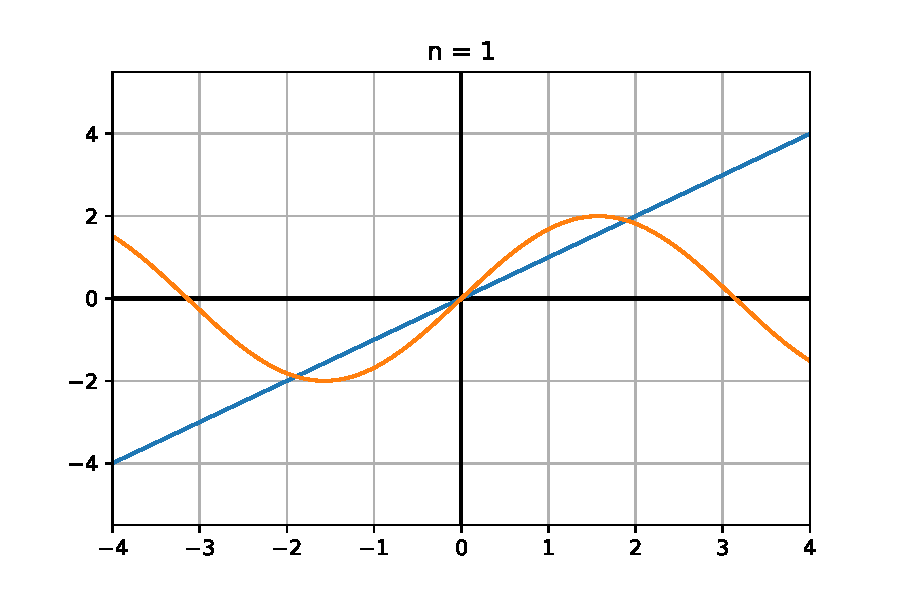
\includegraphics[width=0.45\textwidth]{Fysisk_Matematik/fig/1sin.pdf}
	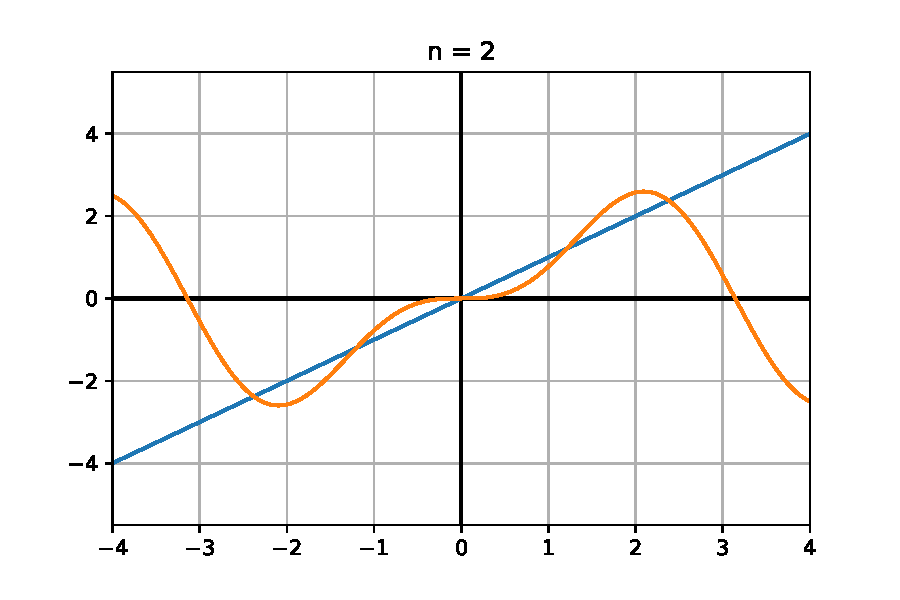
\includegraphics[width=0.45\textwidth]{Fysisk_Matematik/fig/2sin.pdf}
	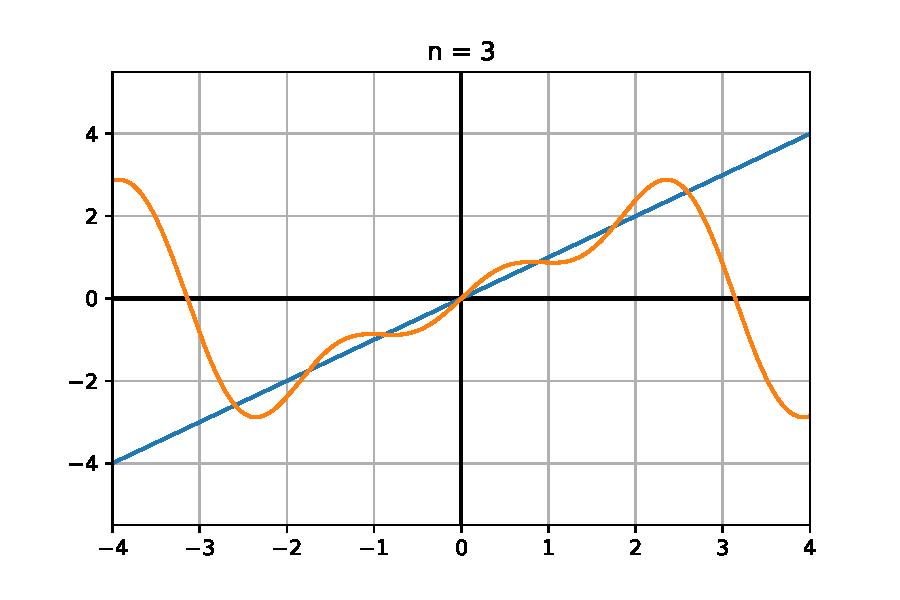
\includegraphics[width=0.45\textwidth]{Fysisk_Matematik/fig/3sin.pdf}
	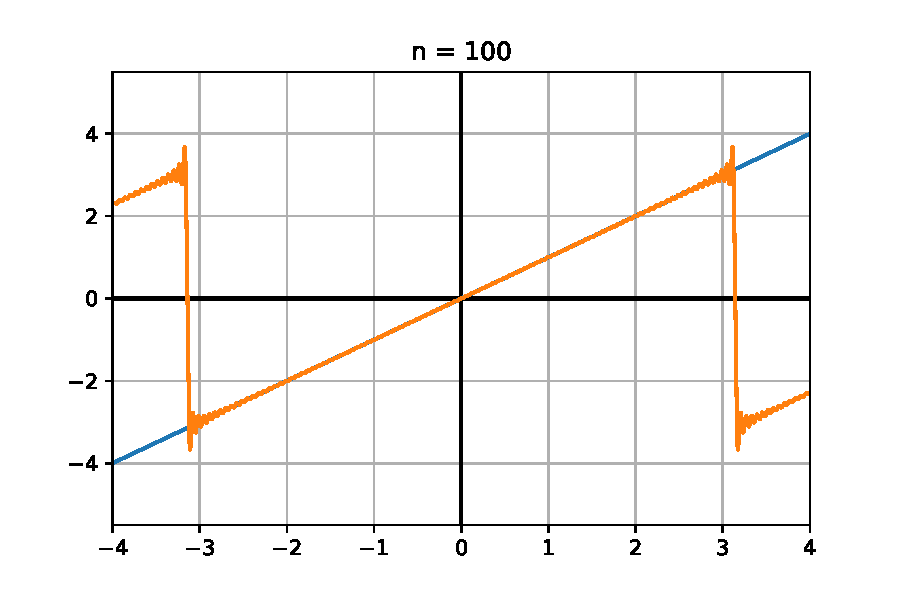
\includegraphics[width=0.45\textwidth]{Fysisk_Matematik/fig/100sin.pdf}
	\caption{En ret linje approksimeret af sinus-funktioner - n angiver her antallet af funktioner lagt sammen.}
	\label{matf:fig:sinapproks}
\end{figure}
Ud fra \cref{matf:fig:sinapproks} kan det ses at jo flere funktioner man ligger sammen, med passende valg af $c_n$, jo nærmere kommer vi til noget der ligner den rette linje. I virkeligheden er rette linjer ikke så slemme at regne med at man ofte ikke rigtig behøver at approksimere dem med andre funktioner, men de virker rigtig godt til at vise hvordan disse approksimationer fungerer. Faktoren $c_n$ bestemmer hvor meget hver individuel sinusfunktion betyder. Det er også lidt svært at få hovedet omkring, så igen kigger vi på det grafisk.
\begin{figure}[H]
	\centering
	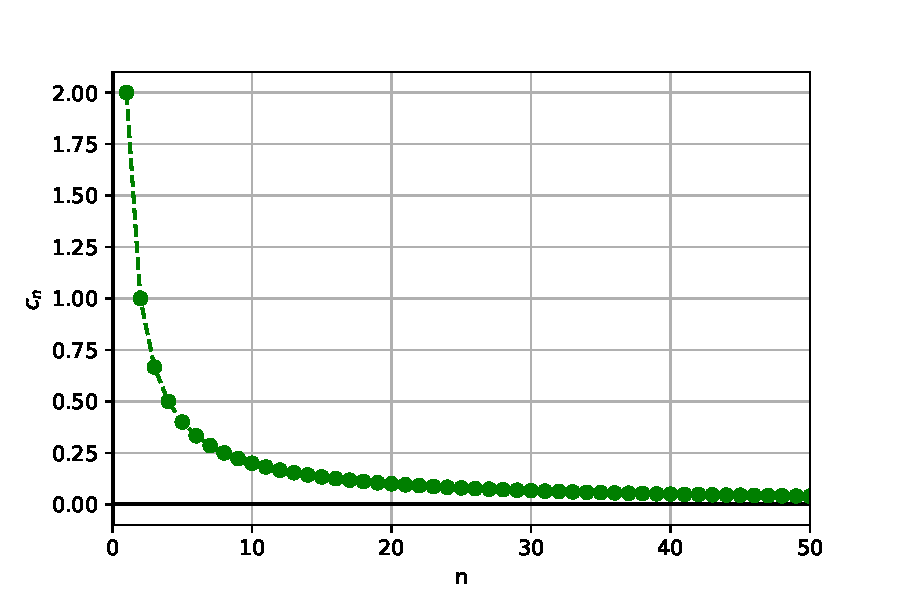
\includegraphics[width=0.6\textwidth]{Fysisk_Matematik/fig/cn.pdf}
	\caption{En graf som viser $|c_n|$ som funktion af $n$. Husk på at $n$ er frekvensen af en given sinusfunktion}
	\label{matf:fig:cn_koeff}
\end{figure}
I \cref{matf:fig:cn_koeff} kan vi se at for den rette linje betyder svingning med frekvens $n=1$ mest, og som $n$ stiger, vil betydning af svingningen falde. Hvordan man helt præcist finder $|c_n|$ kommer vi ikke ind på her, men når vi er færdige med dette kapitel kan har du måske en fornemmelse af hvordan.

Men hvorfor skulle vi kun kigge på svingninger med heltallig frekvens? I stedet for at kigge på en diskret fordeling af $n$, kunne man så ikke lige så godt kigge på \emph{alle} mulige frekvenser mellem $-\infty$ og $\infty$? Jo! Lad os gøre det! For at kunne kende forskel vil vi kalde disse kontinuerte frekvenser for $k$ fremfor $n$. Helt tilbage i \cref{mat:subsec:int} lærte vi at hvis vi tager en sum af uendeligt mange infitesimale ting, bliver det til et integrale:
\begin{align}
    \sum_n^{\infty} c_n\xrightarrow{n\rightarrow k} \int_{-\infty}^{\infty} c(k) \dd{k}
\end{align}
Lig mærke til at $c$ nu er en \emph{funktion} af $k$, fremfor en række af tal. På samme måde kan vi skrive \cref{matf:eq:sinlin} på denne integraleform som:
\begin{align}
    f(x) = \int_{-\infty}^{\infty} c(k) \sin{(k x)} \dd{k}
    \label{matf:eq:sinint}
\end{align}
Sejt! Nu kan vi beskrive enhver funktion som et integrale over frekvenser! Vi har nu kun ét problem... Hvad med cosinus? Det er super smart at kunne beskrive enhver funktion ud fra sinus funktioner, men i fysikken er cosinus svingninger mindst lige så vigtige! Vi vil altså lave det trick vi lige har gjort med sinus, altså at opstille et integral, men for \emph{både} cosinus og sinus. Vi kender heldigvis en funktion som har både sinus og cosinus i sig: \emph{den komplekse eksponentialfunktion}!
\begin{align}
    e^{ik x} = \cos{(k x)} + i\sin{(k x)}
\end{align}
Hvis vi sætter denne funktion ind i stedet for $\sin{(k x)}$ i \cref{matf:eq:sinint} kan vi beskrive enhver funktion udfra både cosinus og sinusfunktioner.
\begin{align}
    f(x) = \frac{1}{\sqrt{2\pi}} \int_{-\infty}^{\infty} \Tilde{f}(k) \cdot e^{ik x} \dd{k}
    \label{matf:eq:invfour}
\end{align}
Når vi laver den her slags integral kalder vi funktionen inde i integralet, altså $\Tilde{f}(k)$, for den \emph{fouriertransformerede} af $f(x)$. Vi kan også omvendt skrive
\begin{align}
    \Tilde{f}(k) = \mathcal{F}\left[f(x)\right] = \frac{1}{\sqrt{2\pi}} \int_{-\infty}^{\infty} f(x) \cdot e^{-ik x} \dd{x}
\end{align}
Processen som omskriver en funktion til dens fouriertransformerede kalder man for en \emph{fouriertransformation}. Som du nok kan forestille dig er det ret svært at lave en fouriertransformation og vi vil derfor ikke gå alt for dybt ind eksempler på fouriertransformationer, men mere fokusere på deres egenskaber og hvordan de hjælper med at løse differentialligninger. 

\subsection{Partiel integration}

For at se hvordan fouriertransformationer hjælper os med at løse differentialligninger, så skal vi først lige lære endnu en måde at integrere, nemlig hvad man kalder \emph{partiel integration}. Det er en teknik man bruger hvis man ønsker at finde integralet af produktet af to funktioner:
\begin{align}
    \int_a^b f(x) g(x) \dd x = \left[G(x) f(x)\right]_a^b - \int_a^b G(x) \dv{f(x)}{x} \dd x
    \label{matf:eq:partdiff}
\end{align}
Her er $G(x)$ stamfunktionen til $g(x)$, altså $G(x) = \int g(x) \dd x$. Vi vil ikke bevise \cref{matf:eq:partdiff} her, da det er ret besværligt. Vi vil bruge et specialtilfælde af partiel integration hvor den ene funktion er et differentiale:
\begin{align}
    \int_a^b f(x) \dv{g(x)}{x} \dd x = \left[g(x) f(x)\right]_a^b - \int_a^b g(x) \dv{f(x)}{x} \dd x
    \label{matf:eq:partdiffdiff}
\end{align}
Lad os kigge på hvad det betyder når vi prøver at løse differentialligninger med fouriertransformationer. Lad os sige at vi har et differentiale som vi prøver at fouriertransformere:
\begin{align}
    \mathcal{F}\left[ \dv{f(x)}{x} \right] = \frac{1}{\sqrt{2\pi}} \int_{-\infty}^{\infty} \dv{f(x)}{x}\cdot e^{-ik x} \dd x
\end{align}
Vi kan nu bruge \cref{matf:eq:partdiffdiff} til at sige:
\begin{align}
    \frac{1}{\sqrt{2\pi}} \int_{-\infty}^{\infty} \dv{f(x)}{x}\cdot e^{-ik x} \dd x = \frac{1}{\sqrt{2\pi}}\left[ f(x) \cdot e^{-ik x}\right]_{-\infty}^{\infty} - \frac{1}{\sqrt{2\pi}}\int_{-\infty}^{\infty}f(x) \dv{e^{-ik x}}{x} \dd x
    \label{matf:eq:partfour}
\end{align}
Lad os starte med at kigge på den første del af dette udtryk:
\begin{align}
    \frac{1}{\sqrt{2\pi}}\left[ f(x) \cdot e^{-ik x}\right]_{-\infty}^{\infty} = \frac{1}{\sqrt{2\pi}}\left( f(\infty)e^{-ik \infty} - f(-\infty)e^{ik \infty} \right)
    \label{matf:eq:inflimits}
\end{align}
Vi kommer her til at lave en antagelse: $f(\infty) = f(-\infty) = 0$. Med dette bliver \cref{matf:eq:inflimits}
\begin{align}
    \frac{1}{\sqrt{2\pi}}\left[ f(x) \cdot e^{-ik x}\right]_{-\infty}^{\infty} = 0
\end{align}
Det kan være lidt svært at forstå hvorfor vi gør det, men tænk på det således: Hvis $f(x)$ ikke blev $0$ i $\infty$ ville hele integralet ikke kunne give noget endeligt, og så ville vi ende med at den fouriertransformerede ville blive uendelig, og det hjælper os ikke så meget. Det betyder så også at funktioner som \emph{ikke} bliver $0$ i $\infty$ ikke kan blive fouriertransformeret. Lad os nu kigge tilbage på \cref{matf:eq:partfour}:
\begin{align}
    \frac{1}{\sqrt{2\pi}} \int_{-\infty}^{\infty} \dv{f(x)}{x}\cdot e^{-ik x} \dd x = - \frac{1}{\sqrt{2\pi}}\int_{-\infty}^{\infty}f(x) \dv{e^{-ik x}}{x} \dd x
    \label{matf:eq:fourlmost}
\end{align}
Eksponentialfunktioner er heldigvis ikke så slemme at differentiere.
\begin{align}
    \dv{e^{-ik x}}{x} = -ik e^{-ik x}
\end{align}
Dette kan vi sætte ind i \cref{matf:eq:fourlmost} og trække konstanterne ude foran integralet, så vi finder
\begin{align}
    \frac{1}{\sqrt{2\pi}} \int_{-\infty}^{\infty} \dv{f(x)}{x}\cdot e^{-ik x} \dd x =  \frac{ik}{\sqrt{2\pi}}\int_{-\infty}^{\infty}f(x) e^{-ik x} \dd x = ik \Tilde{f}(k)
\end{align}
Altså hvis vi har et differentiale som bliver fouriertransformeret, er det det samme som bare at gange den fouriertransformerede med en konstant! Hvis man har et højere ordens differentiale fungerer dette på samme måde, udregningen er bare lidt længere. Man kan altså finde:
\begin{align}
    \mathcal{F}\left[ \dv[2]{f(x)}{x} \right] = (ik)^2 \Tilde{f}(k) = -k\Tilde{f}(k)
    \label{matf:eq:fourtwo}
\end{align}
eller helt generelt:
\begin{align}
    \mathcal{F}\left[ \dv[n]{f(x)}{x} \right] = (ik)^n \Tilde{f}(k)
    \label{matf:eq:fourn}
\end{align}
hvor $n$ er et arbitrært heltal. At vise \cref{matf:eq:fourtwo} og \cref{matf:eq:fourn} overlades som en opgave til læseren.

Okay, men hvordan hjælper det? Lad os prøve at kigge på en partiel differentialligning:
\begin{align}
    \pdv[2]{f(x,t)}{x} = \frac{1}{D}\pdv{f(x,t)}{t}
\end{align}
Hvor $D$ er en konstant. Denne ligning er hvad vi kalder diffusionsligningen, og den kan anvendes til at vise hvordan varme spreder sig i et medium. Vi vil gerne finde løsningen $f(x,t)$. Vi kunne bruge separation af variable, men lad os prøve at anvende hvad vi lige har lært om fouriertransformationer. Det er vigtigt lige at huske på at hvis vi laver en fouriertransformation over én variabel, f.eks. $x$, vil det ikke påvirke den anden variabel $t$. Vi kan altså fouriertransformere én variabel alene. Lad os fouriertransformere denne ligninghvor vi sender $x$ over i $k$.
\begin{align}
    \mathcal{F}\left[ \pdv[2]{f(x,t)}{x} \right] = \mathcal{F}\left[ \frac{1}{D}\pdv{f(x,t)}{t} \right]
    \label{matf:eq:diffuse}
\end{align}
Fra \cref{matf:eq:fourtwo} kan vi se at venstresiden må blive
\begin{align}
    \mathcal{F}\left[ \pdv[2]{f(x,t)}{x} \right] = -k^2 \Tilde{f}(k,t)
\end{align}
Bemærk her at vi ikke har rørt ved $t$. Lad os hernæst kigge på højresiden af \cref{matf:eq:diffuse}. Da en fouriertransformation er et integrale over $x$, kan vi roligt trække både konstanten $\nicefrac{1}{D}$ og differentialet i $t$ ud\footnote{Her ville en matematiker nok protestere og sige at man skal huske at tjekke kontinuitet, men da alle løsninger som giver fysisk mening er kontinuere, så lader vi være.} - altså har vi:
\begin{align}
    \mathcal{F}\left[ \frac{1}{D}\pdv{f(x,t)}{t} \right] = \frac{1}{D}\pdv{}{t}\mathcal{F} \left[ f(x,t) \right] = \frac{1}{D}\pdv{\Tilde{f}(k,t)}{t}
\end{align}
Samler vi begge sider får vi altså:
\begin{align}
    -k^2 \Tilde{f}(k,t) = \frac{1}{D}\pdv{\Tilde{f}(k,t)}{t}
\end{align}
Tada! Vi har nu gjort en partiel differentialligning til en normal differentialligning, blot ved at anvende fouriertrasformationer. Lad os lige rykke $D$ over på den anden side, således at vi har en bedre idé om hvad vi arbejder med. 
\begin{align}
    \pdv{\Tilde{f}(k,t)}{t} = -k^2 D \Tilde{f}(k,t)
\end{align}
Vi ved altså at $\Tilde{f}(k,t)$ er en funktion som giver sig selv ganget med en konstant hvis man differentierer den. Sådan en funktion kender vi heldigvis: en eksponentialfunktion!
\begin{align}
    \Tilde{f}(k,t) = Ae^{-k^2 D t}
\end{align}
Hvor $A$ er en arbitrær konstant.\footnote{Da vi har differentieret med hensyn til $t$ kan $A$ egentlig godt være en arbitrær funktion af $k$, hvis vi lader den være det bliver de følgende udregninger meget langhårede.} Nu har vi altså et udtryk for den fouriertransformerede, så vi kan nu anvende \cref{matf:eq:invfour} til at bestemme $f(x,t)$:
\begin{align}
    f(x,t) = \frac{1}{\sqrt{2\pi}}\int_{-\infty}^{\infty} \Tilde{f}(k,t) e^{ikx} \dd k \\
    = \frac{A}{\sqrt{2\pi}}\int_{-\infty}^{\infty} e^{-k^2 D t} e^{ikx} \dd k = \frac{A}{\sqrt{2\pi}}\int_{-\infty}^{\infty} e^{-k^2 D t + i k x} \dd k
\end{align}
Dette integrale er fuldstændigt urimeligt svært at løse selv, men heldigvis kan man bede en matematiker (eller dit yndlings CAS-værktøj) om at gøre det. Resultatet bliver
\begin{align}
    f(x,t) = \frac{A}{\sqrt{2D t}}e^{-\nicefrac{x^2}{4Dt}}
\end{align}
Sådan kan man altså løse en differentialligning med fouriertransformationer. 

\section{Schrödingerligningen}

Lad os nu tage alt vi har lært om differentialligninger og bruge det til at løse et fysisk problem. Du har måske ude i æteren hørt om kvantemekanik - fysik som beskriver opførslen af meget meget små objekter og partikler. På samme måde som vi i klassisk mekanik har Newtons 2. lov som beskriver alt ved et givet system, bliver alt i et givet system beskrevet ved \emph{Schrödingerligningen}:
\begin{align}
    i\hbar \pdv{\Psi(x,t)}{t} = -\frac{\hbar^2}{2 m}\pdv[2]{\Psi(x,t)}{x} + V(x)\Psi(x,t)
\end{align}
Der er mange versioner af Schrödingerligningen, men den som vi vil arbejde med er den 1-dimensionelle version. Den er lidt lang og fæl at se på, sa lad os tage et kig på de forskellige elementer af den. $\hbar$ (udtalt "h-streg" eller "h-bar") er den reducerede Planck's konstant, en naturkonstant med værdien $\hbar = \SI{1.05e-34}{\joule \second}$. Massen af partiklen man undersøger er angivet med $m$. $i$ er den komplekse enhed som vi kender den. $V(x)$ er potentialfunktionen som beskriver den potentielle energi i systemet. $\Psi(x,t)$ er hvad man kalder bølgefunktionen, og det er her kvantemekanik bliver en smule underligt. Bølgefunktionen for et system beskriver alt hvad der er værd at vide ved systemet, men mere præcist kan du tænke på den som en sandsynlighedsfordeling. Man kan i kvant aldrig vide hvor en partikel er før man kigger, men bølgefunktionen beskriver hvor \emph{sandsynligt} det er at finde partiklen ved et specifikt $x$. Det kan være meget abstrakt at forestille sig, men det vigtige for dette afsnit er ikke så meget at lære kvantemekanik, det vigtige er at løse differentialligninger, så lad os gå i gang med det! Vi vil anvende seperation af variable til at splitte Schrödingerligningen op i en tidsligning og en positionsligning. Altså antager vi at vores løsninger ser således ud:
\begin{align}
    \Psi(x,t) = \psi(x)\phi(t)
\end{align}
Schrödingerligningen bliver således til:
\begin{align}
    i\hbar \psi(x) \pdv{\phi(t)}{t} = -\frac{\hbar^2 \phi(t)}{2m}\pdv[2]{\psi(x)}{x} + V(x)\psi(x)\phi(t)
\end{align}
Vi ganger igennem med $\nicefrac{1}{\psi\phi}$ og får:
\begin{align}
    \frac{i\hbar \psi(x)}{\psi(x) \phi(t)}\pdv{\phi(t)}{t} = - \frac{\hbar^2\phi(t)}{2m \psi(x)\phi(t)}\pdv[2]{\psi(x)}{x} + V(x)\frac{\psi(x)\phi(x)}{\psi(x)\phi(x)}
\end{align}
\begin{align}
    \frac{i\hbar}{\phi(t)}\pdv{\phi(t)}{t} = -\frac{\hbar^2}{2m\psi(x)}\pdv[2]{\psi(x)}{x} + V(x)
    \label{matf:eq:schrod_sep}
\end{align}
Da venstre side nu kun er en funktion af $t$ og højre side kun er en funktion $x$, kan vi igen sige at begge sider må være lig en konstant som vi vil kalde $E$. Lad os starte med at løse venstresiden for $\phi(t)$:
\begin{align}
    \frac{i\hbar}{\phi(t)} \pdv{\phi(t)}{t} = E, \hspace{3mm} \text{eller:} \hspace{3mm} \pdv{\phi(t)}{t} = -\frac{iE}{\hbar}\phi(t)
\end{align}
Husk på at $\nicefrac{1}{i} = -i$. Da $\phi(t)$ differentieret bliver sig selv ganget en konstant, må løsningen være en eksponentialfunktion:
\begin{align}
    \phi(t) = e^{-\nicefrac{iEt}{\hbar}} 
\end{align}
Hermed har vi første del af vores løsning!\footnote{Egentlig ville man også normalt gange en konstant $A$ på, men da vi alligevel ganger $\psi(x)$ på senere, kan vi få konstanten derfra.} Nu til at finde $\psi(x)$, hvortil vi har højresiden af \cref{matf:eq:schrod_sep}:
\begin{align}
    -\frac{\hbar^2}{2m\psi(x)}\pdv[2]{\psi(x)}{x} + V(x) = E
\end{align}
Hvortil vi kan gange igennem med $\psi(x)$ og finde:
\begin{align}
    -\frac{\hbar^2}{2m}\pdv[2]{\psi(x)}{x} + V(x) \psi(x) = E\psi(x)
    \label{matf:eq:1dnotime}
\end{align}
For at gå videre med dette skal vi vide hvad $V(x)$ er, for måden man løser Schrödingerligningen afhænger 100\% af hvordan $V(x)$ ser ud. Eksemplet som vi her vil anvende er hvad man kalder \emph{den uendelige potentialebrønd}, som ser således ud:
\begin{align}
    V(x) =
    \begin{cases} 
      0 &  0 \leq x \leq a \\
      \infty & \text{ellers}
   \end{cases}
\end{align}
Her er $a$ en konstant længde. Hvis et potentiale er uendeligt stort i et punk, betyder det at en given partikel skal have uendelig potentiel energi for at kunne befinde sig i det punkt. Da dette ikke er muligt kan vi konkludere at:
\begin{align}
    \psi(x) = 0 \hspace{3mm} \text{for} \hspace{3mm} x < 0, \hspace{2mm} x > a
\end{align}
Vi kan så kigge på \cref{matf:eq:1dnotime} i intervallet $0\leq x \leq a$, hvor $V(x) = 0$:
\begin{align}
    -\frac{\hbar^2}{2m}\pdv[2]{\psi(x)}{x} = E\psi(x) \rightarrow \pdv[2]{\psi(x)}{x} = -\frac{2mE}{\hbar}\psi(x)
\end{align}
Jamen det er jo næsten til at få tårer i øjnene af! En harmonisk oscillator! Ergo ved vi at $\psi(x)$ må være givet ved følgende:
\begin{align}
    \psi(x) = A\cos{(kx)} + B\sin{(kx)}, \hspace{3mm} k = \frac{\sqrt{2mE}}{\hbar}
\end{align}
Lad os også forsøge at bestemme $A$ og $B$, da vi ved at $\psi(x)$ skal have ramt $0$ når vi når til "væggen" af potentialet - altså der hvor potentialet bliver uendeligt. Vi har altså følgende grænsebetingelser:
\begin{align}
    \psi(x = 0) = \psi(x = a) = 0
\end{align}
Lad os starte med at undersøge $x = 0$:
\begin{align}
    \psi(x=0) = 0 = A\cos{(0)} + B \sin{(0)} = A
\end{align}
Vi konkluderer herudfra at $A = 0$, så vi er efterladt med:
\begin{align}
    \psi(x) = B\sin{(kx)}
    \label{matf:eq:inftpotsol}
\end{align}
Så lad os teste grænsen $x = a$.
\begin{align}
    \psi(x = a) = 0 = B\sin{(ka)}
\end{align}
Vi kunne selvfølgelig løse dette ved at sætte $B = 0$, men da ville vi få $\psi(x) = 0$, og det er ikke en specielt interresant løsning. Det må jo så betyde at $\sin{(ka)} = 0$, men da sinus er en periodisk funktion kan den blive $0$ mange steder:
\begin{align}
    \sin{(n\pi)} = 0, \hspace{3mm} n = 0, 1, 2, ...
\end{align}
men hvilket nulpunkt skal vi så vælge? Hvorfor ikke dem alle sammen? Vi kan altså vælge uendeligt mange værdier af $k$, som vi kan kalde $k_n$, hvorom det gælder at
\begin{align}
    k_n a = n \pi \rightarrow k_n = \frac{\sqrt{2mE_n}}{\hbar} = \frac{n\pi}{a}
\end{align}
Bemærk her at vi har klistret et lille indeks $n$ på $E_n$, som vi også kan vælge uendeligt mange værdier af. Isolerer vi for $E_n$ finder vi:
\begin{align}
    E_n = \frac{n^2 \pi^2 \hbar^2}{2ma^2}
\end{align}
Sætter vi vores værdi for $k_n$ ind i \cref{matf:eq:inftpotsol} finder vi at
\begin{align}
    \psi_n (x) = B\sin{ \left(\frac{n\pi}{a} x\right)}
\end{align}
her har vi også sat et indeks på $\psi_n (x)$, da vi nu altid kan lave en ny løsning, blot ved at ændre på $n$. Man kan finde værdien af $B$ ved at gøre det man kalder at \emph{normalisere} $\psi_n (x)$, men det vil vi ikke gøre i dette afsnit. Du kan som altid gribe fat i en faglig hvis du meget gerne vil vide det. Det endelige resultat bliver at $B = \sqrt{\nicefrac{2}{a}}$, således at vores endelige løsning for $\psi_n(x)$ bliver:
\begin{align}
    \psi_n(x) = \sqrt{\frac{2}{a}} \sin{\left(\frac{n\pi}{a} x\right)}
\end{align}
Bemærk at det at vi har fundet forskellige værdier for $E_n$ betyder at vi også får et indeks på vores tidsløsning:
\begin{align}
    \phi_n (t) = e^{-\nicefrac{iE_n t}{\hbar}}
\end{align}
Vi kan sammensætte dette til en endelig løsning:
\begin{align}
    \Psi_n(x,t) = \psi_n (x) \phi_n(t) = \sqrt{\frac{2}{a}}\sin{\left(\frac{n\pi}{a} x\right)}e^{-\nicefrac{iE_n t}{\hbar}}
\end{align}
Her kommer der så noget helt vildt smart: Schrödingerligningen er lineær! Det betyder at en hvilkensomhelst linearkombination af løsninger $\Psi_n (x)$ også er en løsning til Schrödingerligningen! Ergo kan vi lave en generel løsning $\Psi(x,t)$ som
\begin{align}
    \Psi(x,t) = \sum_{n=1}^{\infty} c_n \Psi_n (x,t)
\end{align}
En tilstand beskrevet som en linearkombination af kendte løsninger kaldes for en \emph{superposition}.
Bum! Nu kan du noget kvant!

\cite{RileyHobson2011}
\cite{Lindstroem2016}
\nocite{griffithsIntroductionQuantumMechanics2005}
\end{document}